\documentclass[12pt]{article}
%%% ========== Package setup ==========
\usepackage{listings}   % Script listing package
\usepackage{wrapfig}    % Wrap Figure or table package
\usepackage{multicol}   % Multicolumn package
\usepackage{pdfpages}   % Include pdf files

%%% ========== Format setup ==========
%% Setup chinese words encoder
\usepackage{xeCJK}
\XeTeXlinebreaklocale "zh"
\XeTeXlinebreakskip = 0pt plus 1pt

%% More word fonts
\usepackage{fontspec}
\setmainfont{Times New Roman}
\renewcommand{\familydefault}{\rmdefault}
\setCJKmainfont{標楷體}

%% Chinese paragraph format
\usepackage{indentfirst}
\setlength{\parindent}{2em}

%% Page margin
\usepackage[a4paper, total={6in,8in}]{geometry}

%%% ========== Document ==========
\begin{document}
\newcommand{\MakeTitlePage}[1]{
\begin{titlepage}
    \begin{center}

        \fontsize{50}{10}
        \selectfont
        Optimal Control

        \vspace{1cm}

        \fontsize{30}{10}
        \selectfont
        Final exam

        \vspace{11cm}

        \begin{tabular}{ r l }
            班級: & 航太四A \\ [10pt]
            姓名: & 吳柏勳 \\ [10pt]
            學號: & 407430635 \\ [10pt]
            座號: & 3 \\ [10pt]
        \end{tabular}

    \end{center}
\end{titlepage}
}
\MakeTitlePage{Midterm}


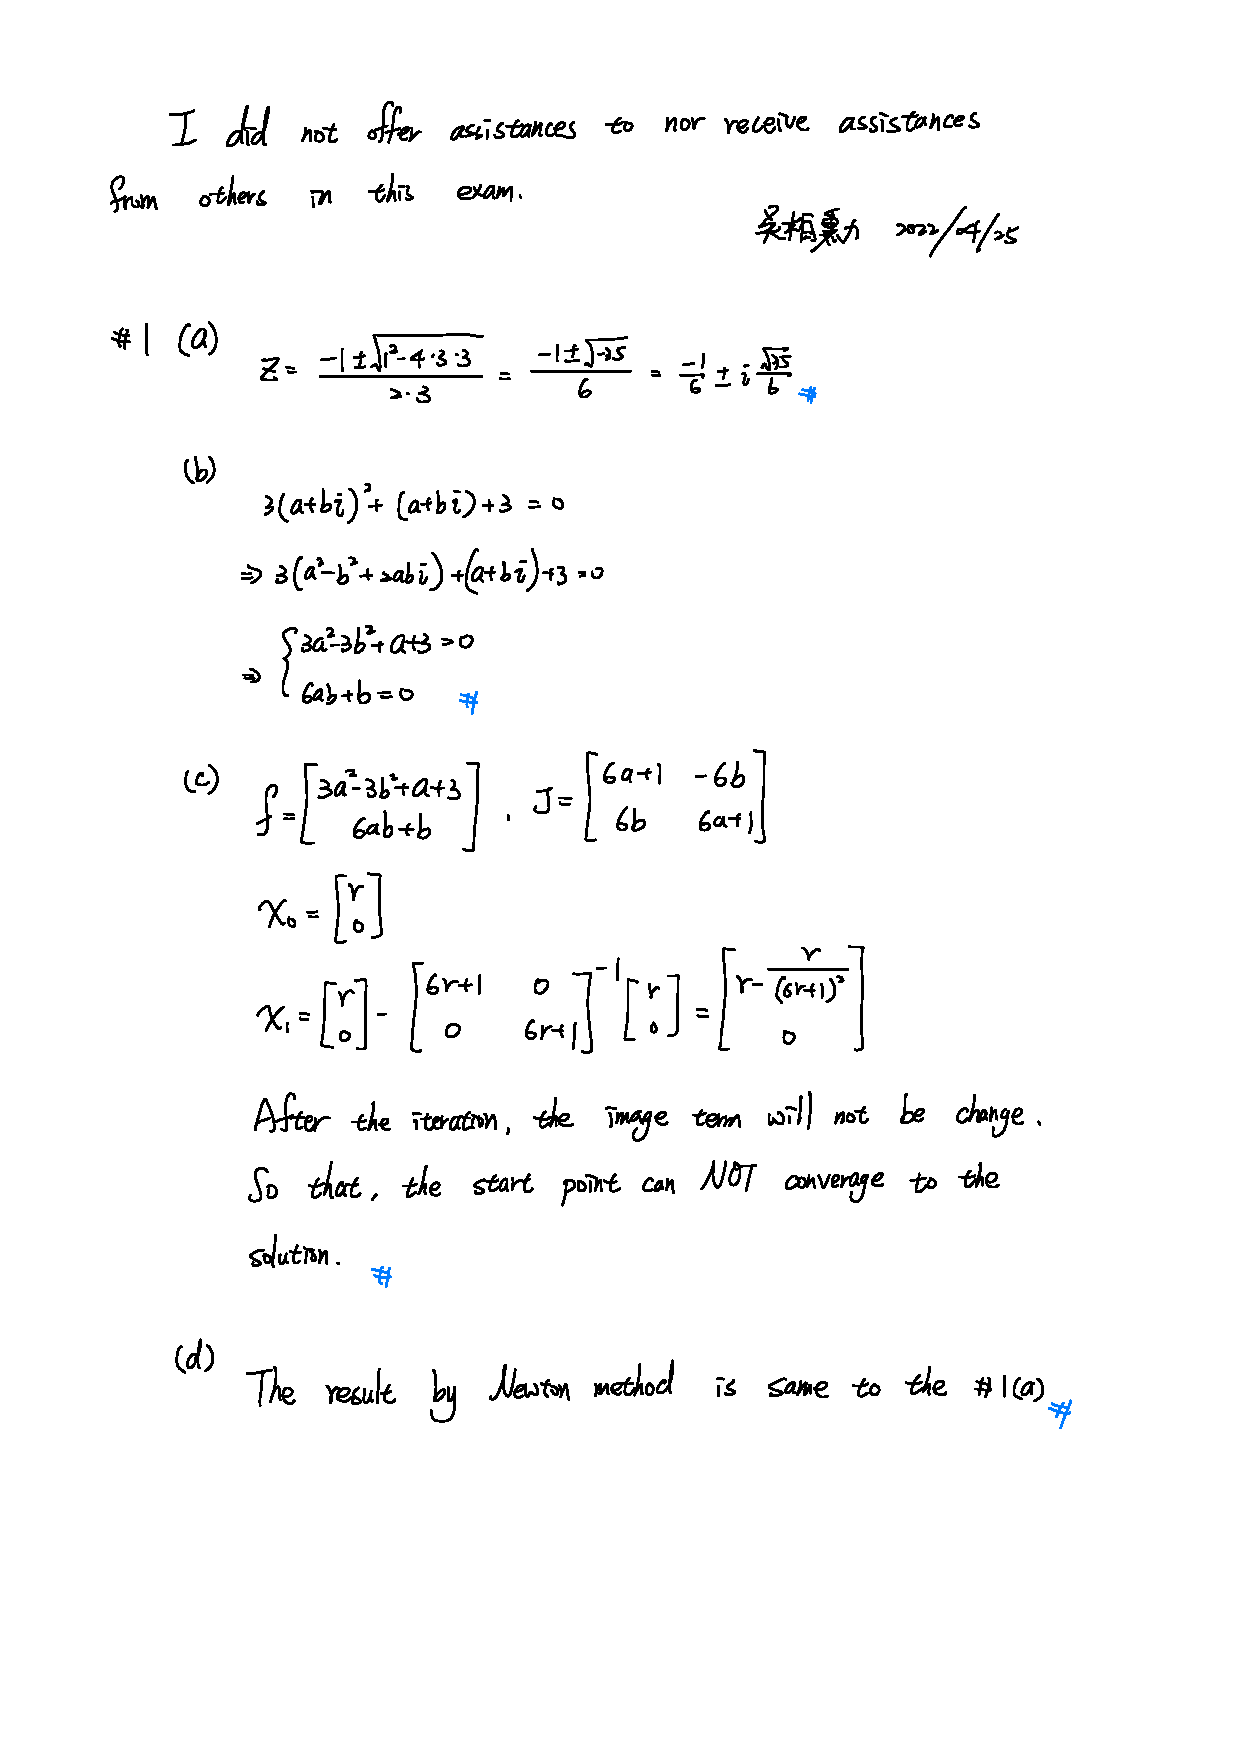
\includepdf[pages=1]{handout.pdf}

\subsection*{\#1(d)}

\begin{verbatim}
clear;clc;close all
syms a b
f = [3*a^2-3*b^2+a+3; 6*a*b+b];
df = [diff(f(1), a), diff(f(1), b)
      diff(f(2), a), diff(f(2), b)];

x = [1; 1];
stop = false;
iter_no = 0;

while ~stop
    delta = -inv(double(subs(df, [a, b], x')))*double(subs(f, [a, b], x'));

    x = x + delta;
    iter_no = iter_no + 1;

    if iter_no >= 100
        stop = true;
    end
end
\end{verbatim}

        \color{lightgray} \begin{verbatim}
x =

   -0.1667
    0.9860

\end{verbatim} \color{black}


\includepdf[pages=2]{handout.pdf}

\subsection*{\#2(b)}

\begin{verbatim}
clear;clc;close all
syms V alpha gamma real
syms T mg lambda1 lambda2 real

ddiff = @(f, x, y) diff(diff(f, x), y);

syms rho S CL_0 CD_0 CL_alpha CD_alpha real
L = 0.5*rho*V^2*S*(CL_0+CL_alpha*alpha);
D = 0.5*rho*V^2*S*(CD_0+CD_alpha*alpha^2);

H = - V*sin(gamma) + lambda1*(T*cos(alpha)-D-mg*sin(gamma)) ...
    + lambda2*(T*sin(alpha)+L-mg*cos(gamma));
Hx = [diff(H, V) diff(H, alpha) diff(H, gamma)];
Hxx = [ddiff(H, V, V)     ddiff(H, V, alpha)     ddiff(H, V, gamma)
       ddiff(H, alpha, V) ddiff(H, alpha, alpha) ddiff(H, alpha, gamma)
       ddiff(H, gamma, V) ddiff(H, gamma, alpha) ddiff(H, gamma, gamma)];
\end{verbatim}


\subsection*{\#2(c)}

\begin{verbatim}
clc;close all
mg_ = 95000*9.81;   S_ = 153;
rho_ = 0.7782;      T_ = 200000;
CL_0_ = 0.3;        CL_alpha_ = 0.1;
CD_0_ = 0.07351;    CD_alpha_ = 0.01;

Hx = subs(Hx, [mg S rho CL_0 CD_0 CL_alpha CD_alpha T], ...
              [mg_ S_ rho_ CL_0_ CD_0_ CL_alpha_ CD_alpha_ T_]);
Hxx = subs(Hxx, [mg S rho CL_0 CD_0 CL_alpha CD_alpha T], ...
                [mg_ S_ rho_ CL_0_ CD_0_ CL_alpha_ CD_alpha_ T_]);

eqn = @(x) double(subs(Hx, [V alpha gamma lambda1 lambda2], x));

opts = optimoptions(@fsolve,'Algorithm', 'levenberg-marquardt', 'Display', 'off');
x = fsolve(eqn, [100 10 20 1 0], opts)
\end{verbatim}

        \color{lightgray} \begin{verbatim}
x =

   99.9864   10.4153   19.7082    0.3536    0.3053
\end{verbatim} \color{black}


\includepdf[pages=3]{handout.pdf}

\end{document}

